\section{Istruzioni all'uso}
Tutte le funzionalità di \NomeProgetto{} sono facilmente reperibili nel menu laterale a comparsa. Per aprirlo basta semplicemente passarci sopra con il cursore.\\
Al primo avvio sono selezionabili solamente le voci che permettono di caricare dei dati o recuperare una sessione di lavoro. Le voci rimanenti sono disabilitate in quanto necessitano dati da elaborare. Questo è visibile all'utente ed è segnalato con un tooltip passando sopra alle varie voci del menù con il cursore.

\subsection{Ripristino sessione}

Cliccando sul pulsante \textit{Carica/Salva Sessione} un utente che aveva precedentemente utilizzato il sito ed esportato una sessione, come spiegato a \S 4.6, può riportare lo stato dell'applicazione a come lo aveva lasciato.
\begin{figure}[H]
		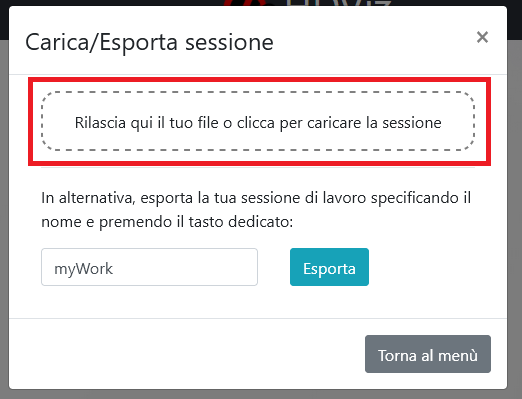
\includegraphics[scale=0.7]{Images/CaricaSessione.png}
		\centering
		\caption{Sezione per il ripristino della sessione}
\end{figure}

Per ripristinare la sessione sarà sufficiente trascinare il file JSON contente la sessione nel riquadro evidenziato in Figura 2, oppure cliccare su tale riquadro e successivamente selezionare il file JSON dal proprio dispositivo. Al termine del ripristino viene notificato il successo dell'operazione o l'eventuale fallimento nel caso il file non sia valido.
Il ripristino della sessione andrà a caricare dimensioni e matrici delle distanze, ottenute tramite riduzioni dimensionali, e tutte le preferenze di visualizzazione nei vari grafici che l'utente aveva utilizzato durante la propria sessione di lavoro. Anche i dati originali sono interessati dal processo di ripristino e non risulta quindi necessario svolgere le azione illustrate a \S 4.2. 

\newpage

\subsection{Caricamento dati}

Tra le voci disponibili al primo avvio dell'applicazione ne sono sono presenti due che possono essere utilizzate per caricare i dati nel sistema:
\begin{itemize}
	\item \textit{Carica dati dal \glo{database}};
	\item \textit{Carica dati da \glo{CSV}}.
\end{itemize}

Entrambe aprono una finestra di dialogo per compiere le operazioni indicate.
Di seguito sono riportati i messaggi d'esito, positivo o negativo, in riferimento all'effettivo caricamento dei dati nel sistema e che saranno mostrati all'utente alla chiusura delle finestre.

	\begin{figure}[H]
		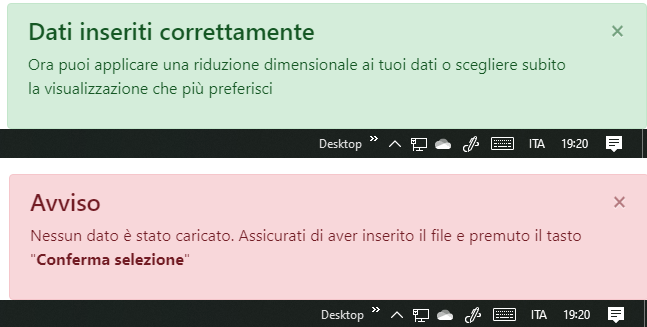
\includegraphics[scale=0.8]{Images/doubleEsito.png}
		\centering
		\caption{Messaggi d'esito del caricamento dati nel sistema}
	\end{figure}
\newpage
\subsubsection{Caricamento dati dal database}
La finestra per il caricamento dei dati dal \glo{database} permette di scegliere uno dei dataset presenti ed effettuare immediatamente una selezione delle dimensioni da caricare.
	
	\begin{figure}[H]
		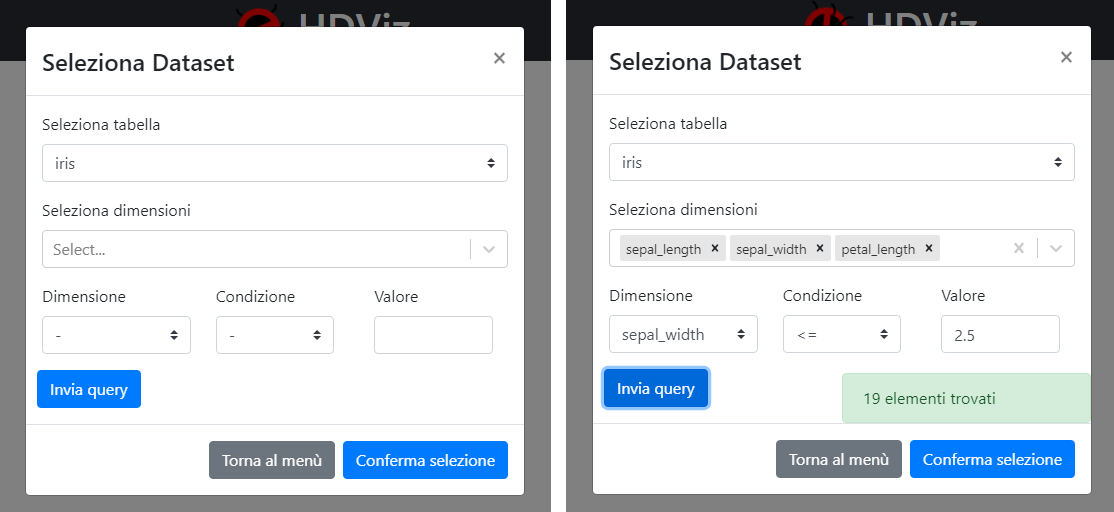
\includegraphics[scale=0.6]{Images/double.png}
		\centering
		\caption{Caricamento dati da database}
	\end{figure}
	
Dopo aver selezionato le dimensioni desiderate dal dataset scelto, premendo il tasto "\textit{Invia\\ query}" verrà visualizzato un messaggio d'esito (positivo o negativo) contente il numero di elementi individuati. L'utente ha la possibilità d'imporre delle condizioni su determinate dimensioni, in modo da prelevare solo particolari punti di suo interesse.\\ Terminata la scrematura dei dati, premendo il tasto "\textit{Conferma selezione}" i dati verranno caricati nel sistema. 
\newpage
\subsubsection{Caricamento dati da CSV}
	La finestra per il caricamento dei dati da file \glo{CSV} presenta una sezione \glo{\textit{drag and drop}} per il caricamento di un file \texttt{.csv} dell'utente; in alternativa, la sezione può essere cliccata per utilizzare l'esplora risorse del proprio dispositivo.\\ Caricato il file, la finestra permette la selezione delle dimensioni che si desidera utilizzare. Di default tutte le dimensioni presenti nel dataset vengono preselezionate e premendo il tasto "\textit{Conferma selezione}" i dati saranno caricati nel sistema.
	\begin{figure}[H]
		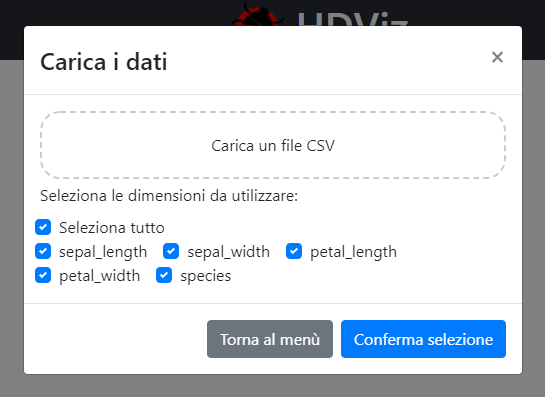
\includegraphics[scale=0.7]{Images/CaricamentoCSV.png}
		\centering
		\caption{Caricamento dati da file CSV}
	\end{figure}

%\begin{figure}[H]
%		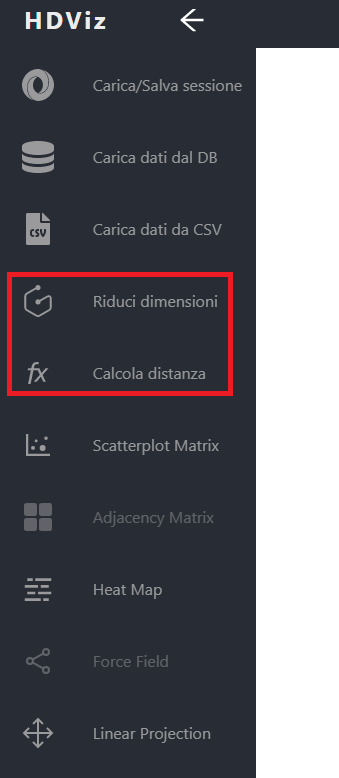
\includegraphics[scale=0.6]{Images/SceltaAlgoritmi.png}
%		\centering
%		\caption{Riduzione dimensionale o calcolo della distanza}
%\end{figure}

\newpage
\subsection{Riduzione dimensionale} 
In seguito al caricamento dei dati vengono rese disponibili ulteriori voci, tra cui "\textit{Riduci dimensioni}". Cliccando su questa voce si apre una finestra che permette di scegliere quali dimensioni saranno interessate dal processo, se normalizzare o meno i dati e quale algoritmo utilizzare tra:

\begin{itemize}
	\item \glo{FastMap};
	\item \glo{PCA};
	\item \glo{LLE};
	\item \glo{IsoMap};
	\item \glo{t-SNE};
	\item \glo{UMAP}.
\end{itemize}

In base a questa ultima scelta l'utente potrà selezionare una serie di parametri specifici per eseguire la riduzione come più preferisce.

\begin{figure}[H]
		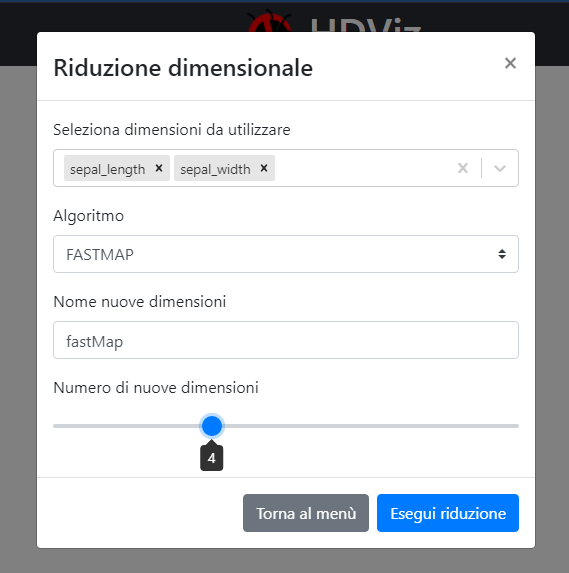
\includegraphics[scale=0.65]{Images/RiduzioneDimensionale.png}
		\centering
		\caption{Finestra per la riduzione dimensionale tramite algoritmo}
\end{figure}

Ultimata la configurazione, premendo il tasto "\textit{Esegui riduzione}" verranno create ed inserite le nuove dimensioni nel sistema.

\newpage
\subsection{Calcolo della distanza}
In seguito al caricamento dei dati vengono rese disponibili ulteriori voci, tra cui "\textit{Calcola distanza}". Cliccando su questa voce si apre una finestra che permette di scegliere quali dimensioni utilizzare per creare una matrice delle distanze, quale nome assegnarvi, se normalizzare o meno i dati e quale funzione di distanza usare tra:

\begin{itemize}
	\item \glo{Euclidea};
	\item \glo{Canberra};
	\item \glo{Chebyshev};
	\item \glo{Manhattan}.
\end{itemize}

\begin{figure}[H]
		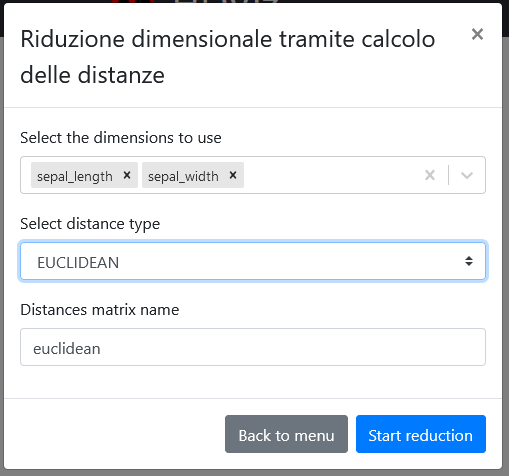
\includegraphics[scale=0.65]{Images/CalcoloDistanze.png}
		\centering
		\caption{Finestra per la riduzione dimensionale tramite il calcolo delle distanze}
\end{figure}

Terminata la configurazione, premendo il tasto "\textit{Esegui riduzione}" verrà creata la matrice e salvata nel sistema. Le matrici create dall'utente saranno disponibili in tutti i grafici che dipendono dal concetto di distanza (come Adjacency Matrix e Force Field).

\newpage
\subsection{Scelta del grafico e visualizzazione dei dati}
Una volta elaborati i dati o eventualmente immediatamente dopo al caricamento dei dati, si può scegliere il grafico che più si preferisce tra quelli proposti:
\begin{itemize}
	\item \glo{Scatterplot matrix};
	\item \glo{Adjency matrix};
	\item \glo{Heat map};
	\item \glo{Force field};
	\item \glo{PLMA (Proiezione lineare multi asse)}.
\end{itemize}

%\begin{figure}[H]
%		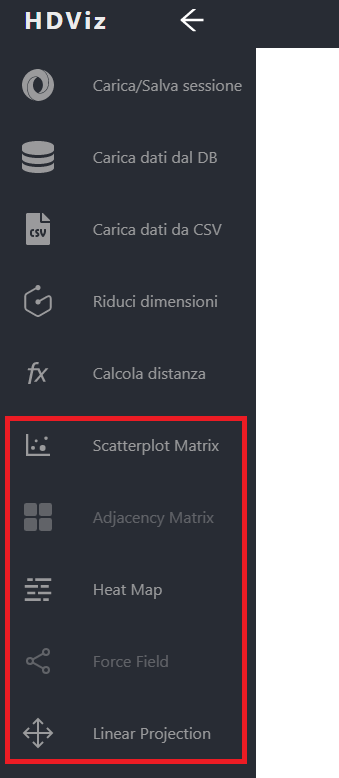
\includegraphics[scale=0.6]{Images/OptionList.png}
%		\centering
%		\caption{Lista dei grafici che è possibile scegliere}
%\end{figure}
Una volta selezionata una di queste opzioni, si aprirà una \glo{form} sulla destra attraverso la quale sarà possibile modificare la visualizzazione del grafico. Inizialmente tutti i campi sono impostati a "\textit{Nessuna dimensione}" quindi è corretto che il grafico non sia già visualizzato. È necessario modificare tali campi a proprio piacimento. Ad ogni loro modifica la visualizzazione cambierà dinamicamente, adattandosi alle dimensioni del dispositivo. La form è inoltre sempre accompagnata da un bottone per nasconderla e centrare il grafico nello schermo per concentrarsi solamente sull'analisi del grafico. 

\newpage

\subsubsection{Scatterplot matrix}

Per questa visualizzazione la \glo{form} a destra permette di:
\begin{itemize}
	\item Modificare le dimensioni da applicare agli assi;
	\item Modificare la dimensione per l'applicazione del colore sui punti.
\end{itemize} 

\begin{figure}[H]
		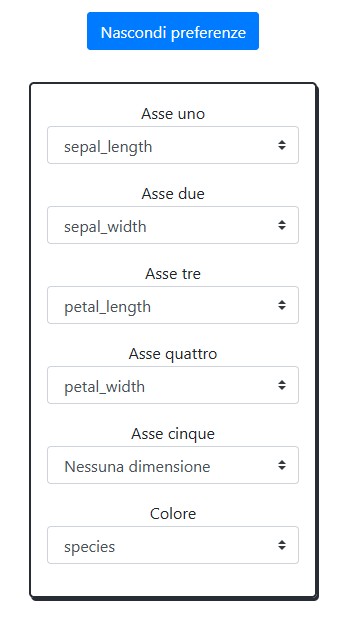
\includegraphics[scale=0.7]{Images/spmp.png}
		\centering
		\caption{Form delle preferenze per il grafico Scatterplot Matrix}
\end{figure}

\newpage
Di seguito un esempio di visualizzazione dei dati con questo grafico.

\begin{figure}[H]
		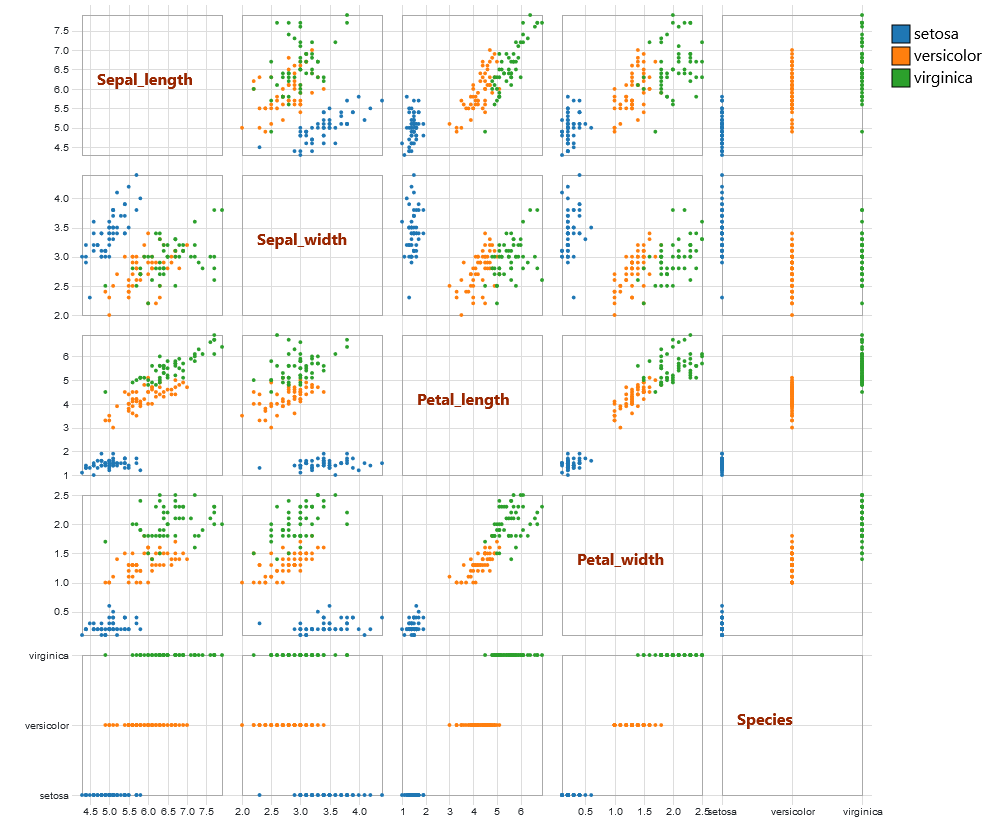
\includegraphics[scale=0.6]{Images/ScatterplotMatrix.png}
		\centering
		\caption{Esempio di visualizzazione dei dati con il grafico Scatterplot Matrix}
\end{figure}

Come visibile in figura, in alto a destra sarà sempre disponibile una legenda dei colori per aiutare l'utente nell'analisi del grafico.\\\mbox{}\\ \textbf{NB}: la legenda sarà disponibile solo dopo aver associato una dimensione al colore dei punti dalla form delle preferenze.

\newpage

\subsubsection{Adjacency matrix}

Per questa visualizzazione la \glo{form} a destra permette di:
\begin{itemize}
	\item Se presente, scegliere una delle matrici delle distanze create dall'utente;
	\item Scegliere per quale dimensione ordinare i punti del grafico;
	\item Scegliere quale dimensione associare alle etichette del grafico;
	\item La distanza minima e massima tra i punti.
\end{itemize} 

\begin{figure}[H]
		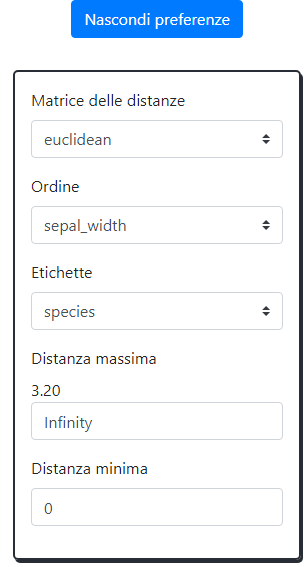
\includegraphics[scale=0.7]{Images/amp.png}
		\centering
		\caption{Form delle preferenze per il grafico Adjacency Matrix}
\end{figure}

\newpage
Di seguito un esempio di visualizzazione dei dati con questo grafico.

\begin{figure}[H]
		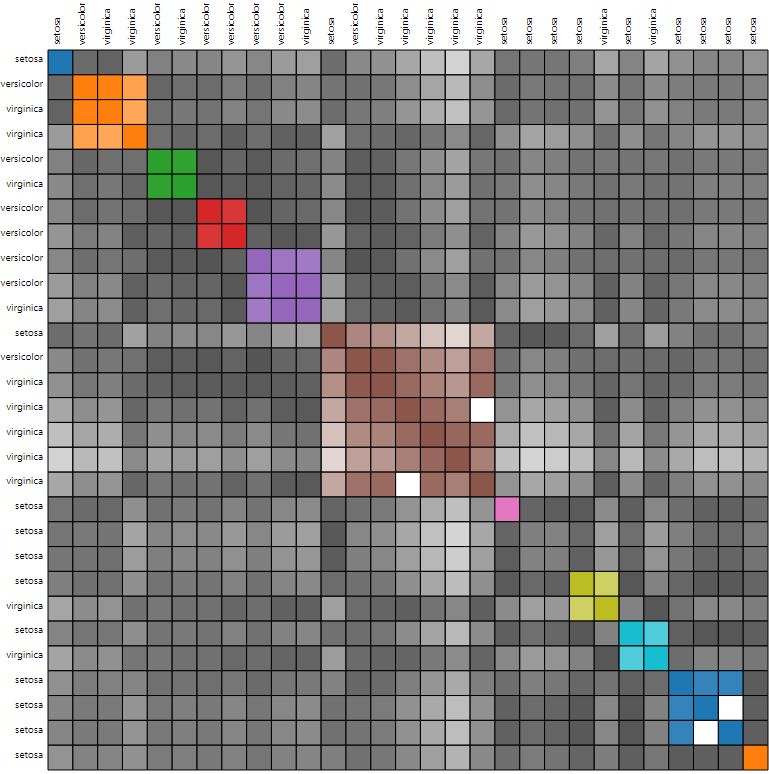
\includegraphics[scale=0.6]{Images/am.png}
		\centering
		\caption{Esempio di visualizzazione dei dati con il grafico Adjacency Matrix}
\end{figure}

\newpage

\subsubsection{Heat map}

Per questa visualizzazione la \glo{form} a destra permette di:
\begin{itemize}
	\item Modificare le dimensioni da applicare agli assi \textit{X} e \textit{Y};
	\item Modificare la dimensione per l'applicazione della scala di colori.
\end{itemize} 

\begin{figure}[H]
		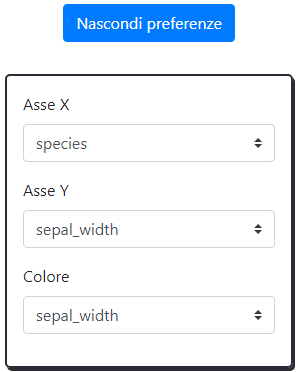
\includegraphics[scale=0.6]{Images/hmp.png}
		\centering
		\caption{Form delle preferenze per il grafico Heat Map}
\end{figure}
Di seguito un esempio di visualizzazione dei dati con questo grafico.

\begin{figure}[H]
		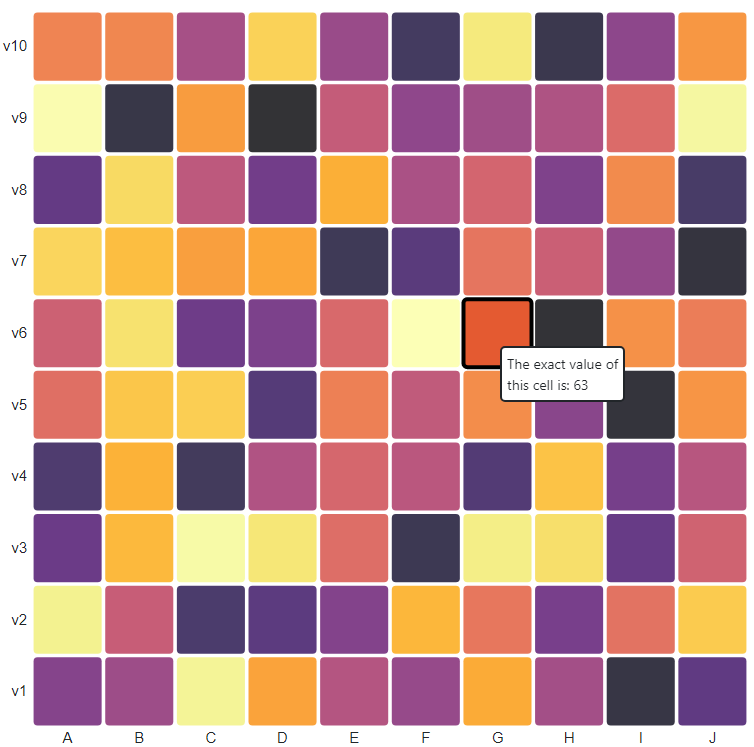
\includegraphics[scale=0.4]{Images/hmb.png}
		\centering
		\caption{Esempio di visualizzazione dei dati con il grafico Heat Map}
\end{figure}

Come visibile nella figura precedente, l'utente potrà visualizzare il valore di ogni cella posizionandosi sopra con il cursore. Tale finestra seguirà il movimento del cursore stesso, per sparire una volta posizionato al di fuori del grafico.

\newpage

\subsubsection{Force field}

Per questa visualizzazione la \glo{form} a destra permette di:
\begin{itemize}
	\item Se presente, scegliere una delle matrici delle distanze create dall'utente;
	\item Scegliere quale dimensione associare al colore dei nodi del grafico;
	\item La distanza minima e massima tra i punti.
\end{itemize} 
Di seguito un esempio di visualizzazione dei dati con questo grafico e relativa form delle preferenze.

\begin{figure}[H]
		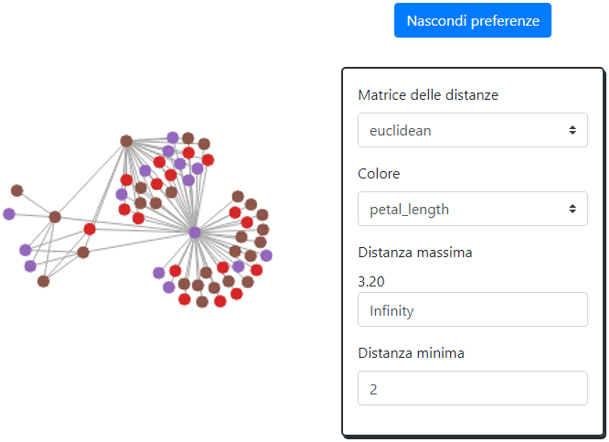
\includegraphics[scale=0.8]{Images/ffpf.png}
		\centering
		\caption{Form delle preferenze per il grafico Force Field ed esempio di visualizzazione}
\end{figure}
I nodi generati possono essere selezionati e spostati nello spazio tridimensionale
per analizzare meglio il contenuto del grafico.

\newpage
\subsubsection{Proiezione lineare multi asse}

Per questa visualizzazione la \glo{form} a destra permette di:
\begin{itemize}
	\item Scegliere le dimensioni d'aggiungere alla visualizzazione;
	\item Scegliere la dimensione d'associare al colore dei punti.
\end{itemize} 

Di seguito un esempio di visualizzazione dei dati con questo grafico e relativa form delle preferenze.
\begin{figure}[H]
		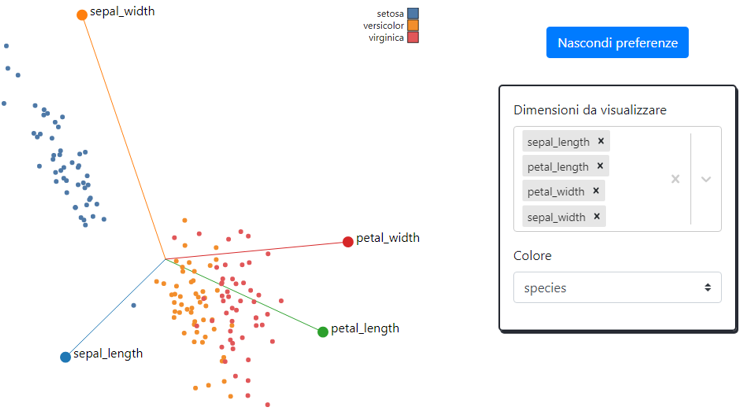
\includegraphics[scale=0.9]{Images/plmad.png}
		\centering
		\caption{Form delle preferenze per il grafico PLMA ed esempio di visualizzazione}
\end{figure}

Gli assi generati possono essere selezionati e spostati per muovere i punti nello spazio tridimensionale e analizzare meglio il contenuto del grafico. \\
Come visibile in figura, in alto a destra sarà sempre disponibile una legenda dei colori per aiutare l'utente nell'analisi del grafico.\\\mbox{}\\ \textbf{NB}: la legenda sarà disponibile solo dopo aver associato una dimensione al colore dei punti dalla form delle preferenze.\\
\mbox{}\\

\newpage
\subsection{Esportazione della sessione}
Nel caso in cui l'utente desidera salvare lo stato dell'applicazione, nel menu è disponibile la voce \textit{Carica/Salva sessione}. L'applicazione permette di esportare lo stato attuale tramite il download di un file in formato JSON che potrà successivamente essere ripristinato (vedere \S 4.1).
\begin{figure}[H]
		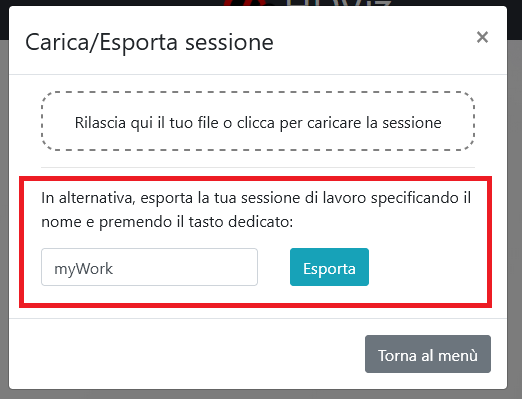
\includegraphics[scale=0.8]{Images/EsportaSessione.png}
		\centering
		\caption{Sezione per l'esportazione della sessione}
\end{figure}
Per esportare la sessione di lavoro l'utente può associare un nome al file e successivamente premere sul pulsante \textit{Esporta}. Il download partirà automaticamente e il file sarà disponibile nel dispositivo utilizzato.
\newpage
\subsection{Formattazione dei file}

Il file in formato CSV da dare in input all'applicazione dovrà seguire la formattazione standard per questo tipo di estensione. In particolare:
\begin{itemize}
	\item La prima riga deve contenere il nome delle dimensioni, separato da una virgola l'una dall'altra;
	\item Le righe successive devono contenere i dati, rispettando l'ordine imposto dalla riga delle dimensioni e separando anch'essi con una virgola l'uno dall'altro;
	\item Al termine della riga andare a capo senza virgola.
\end{itemize}

\textbf{NB}: non è necessario inserire spazi.\\ \mbox{}\\

Di seguito viene riportato un esempio di file CSV formattato correttamente.

\begin{figure}[H]
		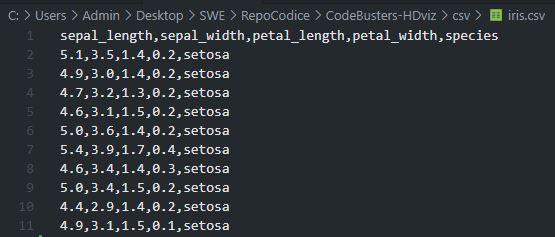
\includegraphics[scale=0.9]{Images/csv}
		\centering
		\caption{Esempio di file CSV correttamente formattato}
\end{figure}